\chapter{Implementation}
This chapter focus mainly about the software implementation for semi-automated detection of sanitization, authentication and declassification errors in UML state Charts. Used Eclipse xtext to develop source code editor, Eclipse xtend to develop source code generator, YAKINDU SCT editor for modeling C/C++ programs as UML statchart and extended static analysis engine named smtcodan using Java, Graphics2D and Jframe. 

\section{Overview of System Architecture}

\begin{figure}[htbp]
	\centering
	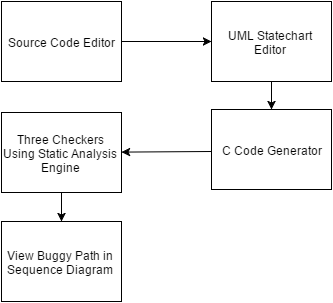
\includegraphics{styles/system_architecture.png}
	\caption{System Overview}
\end{figure}

Figure 4.1 depicts the complete system architecture. First, the source code editor is developed using Eclipse Xtext. By this editor one can easily annotate the source code of C/C++. Even it is possible to annotate C/C++ header files. For information flow vulnerabilities detection in C/C++ code annotation technique has chosen which is easy to extend and backward compatible. Then for modeling purpose Yakindu SCT editor \cite{ref_15_yakindu:sct} has chosen to model the C/C++ code into state charts to detect the bug during design stage of software development life-cycle. Inside the Yakindu SCT editor the annotation language grammar has also included using Eclipse Xtext. So, that user can easily annotate the state charts to detect the information flow vulnerabilities. Afterwards the C code generator has extended inside the Yakindu SCT editor using Eclipse Xtend. After modeling the C code files in Yakindu SCT editor user can easily generate the code using C code generator. Through this generator two files will be generated. One file has .c extension and another file has .h extension. Inside those files annotation has also included. Those annotations are helpful to detect the information flow errors. After generating the code files using static analysis engine named \enquote{smtcodan} three checkers have included to detect authentication, declassification and sanitization function missing vulnerabilities. Then to view the buggy path in sequence diagram a sequence diagram generator has created. That is the end of complete system architecture of this system. 


\section{The Grammar of Annotation Language}

The grammar of annotation language is represented as in Extended Backus Naur Form (EBNF) in Figure \ref{language grammar}. The following type face conventions were used: Italic font for non-terminals, bold typewriter font for literal terminals including keywords.\\
 
 \begin{figure}[ht!]
 	\centering
 	\begin{tabular}{lll}
 		
 		\footnotesize                       
 		\textit{Ann\_Lang}           &\footnotesize $::=$         &\footnotesize HeaderModel*;       \\ \\
 		
 		\footnotesize
 		\textit{H\_Model}            &\footnotesize $::=$         &\footnotesize \textit{S\_L\_Anno};       \hfill ;single line comment rule   \\     
 		&\footnotesize $\ \vert $    &\footnotesize \textit{M\_L\_Anno};       \hfill ;multi line comment rule    \\ 
 		&\footnotesize $\ \vert $    &\footnotesize \textit{Func\_Decl};       \hfill ;function declaration rule  \\ 
 		&\footnotesize $\ \vert $    &\footnotesize \textit{Attr\_Def};        \hfill ;variable declaration rule  \\ \\
 		\footnotesize  	
 		\textit{S\_L\_Anno}          &\footnotesize $::=$         &\footnotesize \textbf{"//@ @function "},    Func\_Type,              [\textbf{H} $\ \vert $  \textbf{L}];     \\
 		&\footnotesize $\ \vert $    &\footnotesize \textbf{"//@ @parameter "},   p\_Name,  Sec\_Type, Var\_Type,    [\textbf{H} $\ \vert $  \textbf{L}];    \\
 		&\footnotesize $\ \vert $    &\footnotesize \textbf{"//@ @variable "},    v\_Name,  Sec\_Type,     [\textbf{H} $\ \vert $  \textbf{L}];    \\
 		&\footnotesize $\ \vert $    &\footnotesize \textbf{"//@ @preStep "},     pr\_s\_Name,             [\textbf{H} $\ \vert $  \textbf{L}];    \\
 		&\footnotesize $\ \vert $    &\footnotesize \textbf{"//@ @postStep "},    po\_s\_Name,             [\textbf{H} $\ \vert $  \textbf{L}];    \\ \\   
 		\footnotesize            
 		\textit{M\_L\_Anno}          &\footnotesize $::=$         &\footnotesize [\textbf{"/*@ "}],  ["* "],  Func\_Ann,  (\textbf{" @*/"}) \\
 		&\footnotesize $\ \vert $    &\footnotesize ("*"), [" "]*, (\textbf{"@*/"});                  \\ \\
 		\footnotesize        
 		\textit{Func\_Ann}           &\footnotesize $::=$         &\footnotesize \textbf{"@function "},    Func\_Type,              [\textbf{H} $\ \vert $  \textbf{L}];     \\
 		&\footnotesize $\ \vert $    &\footnotesize \textbf{"@parameter "},   p\_Name,  Sec\_Type, Var\_Type,    [\textbf{H} $\ \vert $  \textbf{L}];    \\
 		&\footnotesize $\ \vert $    &\footnotesize \textbf{"@preStep "},     pr\_s\_Name,             [\textbf{H} $\ \vert $  \textbf{L}];    \\
 		&\footnotesize $\ \vert $    &\footnotesize \textbf{"@postStep "},    po\_s\_Name,             [\textbf{H} $\ \vert $  \textbf{L}];    \\ \\                                        
 		\footnotesize                       
 		\textit{Func\_Type}          &\footnotesize $::=$        &\footnotesize \textbf{authentication};\\
 		&\footnotesize $\ \vert $ &\footnotesize \textbf{declassification}; \\
 		&\footnotesize $\ \vert $    &\footnotesize \textbf{sanitization};     \\
 		&\footnotesize $\ \vert $    &\footnotesize \textbf{sink};             \\
 		&\footnotesize $\ \vert $    &\footnotesize \textbf{source};           \\
 		&\footnotesize $\ \vert $    &\footnotesize \textbf{trust\_boundary};  \\ \\
 		\footnotesize                       
 		\textit{Sec\_Type}           &\footnotesize $::=$         &\footnotesize \textbf{confidential}; \\
 		&\footnotesize $\ \vert $    &\footnotesize \textbf{source};    \\ \\
 		\footnotesize                       
 		\textit{Var\_Type}           &\footnotesize $::=$         &\footnotesize \textbf{authenticated}; \\
 		&\footnotesize $\ \vert $    &\footnotesize \textbf{declassified}
 		\\
 		&\footnotesize $\ \vert $    &\footnotesize \textbf{sanitized};    \\ \\	
 		
 	\end{tabular}
 	\caption{Light-weight annotation language grammar excerpt}
 	\label{language grammar}
 \end{figure}
 
Annotation language grammar has two grammar rules
\texttt{S\_L\_Anno} and \texttt{M\_L\_Anno} used for defining security annotations. The \texttt{Func\_Decl} and \texttt{Attr\_Definition} rules are used to recognize C or C++ function declarations and variable. The \texttt{Var\_Type} rule is used for variable type which is either for authenticated or declassified or sanitized variable. \texttt{Sec\_Type} rule is used for type of security whether a variable is confidential or not. In \texttt{Func\_Decl} rule the type function is declared. A function can be either one of this like authentication, declassification, sanitization, source or sink.\\



\section{UML State Chart Editor}

A set of formal representation of UML statecharts is presented in this section. The state identifier and event are represented as S and Event respectively both as set types. For simple specification, the basic set types are used. In the definition of a transition from one state to another the guard is defined as a Boolean type. According to F Alhumaidan state based static and dynamic formal analysis of UML state diagrams \cite{ref_16_alhumaidan2012state} , a state can have three possible values that are active, passive or null represented as Active, Passive and null respectively. The type of state can be simple, concurrent, non-concurrent, initial or final.

\begin{figure}[ht!]
	\centering
	\begin{tabular}{lll}
		\footnotesize                       
		\textit{[S, Event]}          &\footnotesize \\
		
		\footnotesize
		\textit{Boolean}            &\footnotesize $::=$         &\footnotesize \textit{True} $\ \vert $ {False};       \\   
		\footnotesize
		\textit{Status}            &\footnotesize $::=$         &\footnotesize \textit{Active}
		 $\ \vert $ {Passive}$\ \vert $ {Null};       \\ 
		\footnotesize
		\textit{Type}            &\footnotesize $::=$         &\footnotesize \textit{Simple}
		 	$\ \vert $ {Concurent}$\ \vert $ {Nonconcurent} $\ \vert $ {Initial}$\ \vert $ {Final};       \\
		 	 
		
	\end{tabular}
	\caption{UML Statechart Formal Representation}
	\label{statechart_formal_representation}
\end{figure}
In modeling using sets, it's not imposing any restriction upon the number of elements and a high level of
abstraction is supposed. Further, it's not insist upon any
effective procedure for deciding whether an arbitrary
element is a member of the given collection or not. As a
consequent, sets S and Event are sets over which cannot define any operation of set theory. For example,
cardinality to know the number of elements in a set cannot
be defined. Similarly, the subset, union, intersection or
complement operations over the sets are not defined.\\

The state diagram is a collection of states related by
certain types of relations. In the definition of a state, state identifier, its type, status and set of regions is required.Region is defined as a power set of sequence of states. The state is represented by a schema which consists of four components described above. All these components are
encapsulated and put in the Schema State given below.
The invariants over the schema are defined in the second
part of schema.\\

\begin{figure}[ht!]
	\centering
	\begin{tabular}{lll}
		\footnotesize                       
		\textit{State}       \\
		
		\footnotesize
		\textit{name}   $:$    \textit{S}  \\   
		\footnotesize
		\textit{type}   $:$    \textit{Type}  \\   
		\footnotesize
		\textit{status}   $:$    \textit{Status}      \\
		\footnotesize
		\textit{regions} $:$   \textit{seq Regions} \\
		
		\footnotesize
		\textit{regions} $=$   \textit{1} $\ \  $ {type}$=$   \textit{Simple} \\
		\footnotesize
		 \textit{\# regions} $=$   \textit{1} $\ \  $ {type}$=$   \textit{Nonconcurrent} \\
		 \textit{\# regions} $=$   \textit{1} $\ \  $ {type}$=$   \textit{Concurent} \\
		 
		
	\end{tabular}
	\caption{UML statechart some other formal representation}
	\label{statechart_formal_representation_part2}
\end{figure}

\textbf{Invariants:}
\begin{itemize}
\item  If there is no region in a state inside the state diagram, then it is a simple state.
\item  If there is exactly one region in a state then it is termed as non-concurrent composite state.
\item  If there are two or more regions in a state then it is
concurrent composite state.
\end{itemize}

The collection of states is represented by the schema
States which consists of four variables. The mapping
substates from State to power set of State describes type
of a state.
 \begin{figure}[ht!]
 	\centering
 	\begin{tabular}{lll}
 		\footnotesize                       
 		\textit{States}          \\
 		\footnotesize                       
 		\textit{start}          
 		$:$  \textit{State}\\
 		
 		\textit{states}          
 		$:$  \textit{State}\\
 		
 		\textit{states}           
 		$:$  \textit{State}\\
 		\footnotesize
 		\textit{substates}            $:$         \textit{State} $\ \  $ {State};       \\   
 		\footnotesize
 		\textit{target}             $:$         \textit{State}    \\
 		 \footnotesize                       
 		 \textit{start}           
 		 $:$  \textit{states}\\
 		  \footnotesize                       
 		  \textit{start}          
 		  $:$ \textit{target}\\
 		   \footnotesize                       
 		   \textit{start}           
 		   $:$  \textit{dom} $\ \  ${substates}\\
 		   
 		   \footnotesize                       
 		   \textit{states}          \\ 		
 		$\ \  $ \textit{s}      $:$     \textit{State} $\ \  $ {s} $\ \  $ \textit{dom} $\ \  ${substates} $\ \  $ {s} $\ \  $ \textit{states}        \\ 
 		$\ \  $ \textit{s}      $:$     \textit{State} $\ \  $ {s} $\ \  $ \textit{states} $\ \  $ {s} $\ \  $ \textit{start} $\ \  $ {s} $\ \  $ \textit{target}$\ \  $ {s.typ}\\ 
 		$\ \  $ \textit{Simple} $\ \  $ {s} $\ \  $ \textit{dom} $\ \  ${substates}\\
 		\footnotesize                       
 		\textit{target}  $\ \  $ \textit{states}        \\ 
 		\footnotesize                       
 		\textit{target}  $\ \  $ \textit{dom} $\ \  ${substates}\\	
 	\end{tabular}
 	\caption{UML Statechart Formal Representation some parts}
 	\label{statechart_formal_representation_invariants}
 	\end{figure}

\textbf{Invariants:}
\begin{itemize}
\item The start state is not in the collection of states.
\item The start state is not the target state.
\item The start state does not belong to domain of substates
mapping that is it has no sub-state.
\item The set of states is non-empty.
\item For any state, s, if it is in the states and is not the start or target state and not the simple state then it belongs to domain of sub-states.
\item The target state does not belong to states.
\item The target state of the state diagram does not belong to domain of the sub-states.
\end{itemize}

UML state chart editor has been extended based on the open source Yakindu SCT \cite{ref_15_yakindu:sct}framework. The existing language grammar with
annotation language grammar has extended in order to support new set
of tags. Furthermore, an annotation proposal filter implemented which was used to filter out the annotation language tags of the Yakindu SCT language grammar.\\

To extend the Yakindu SCT editor here it has been decided to represent the statements like variable declaration, function calling as state and transitions are represent as move from one statement to another. A rectangular box can be attached with transitions where annotation can be written as per requirements. So for the developed system the UML statechart formal representation is as like this: 
\begin{figure}[ht!]
	\centering
	\begin{tabular}{lll}
	\footnotesize                       
	\textit{States}          \\
	\footnotesize                       
	\textit{start}          
	$:$  \textit{State}\\
	
	\textit{states}          
	$:$  \textit{State}\\
	
	\textit{states}           
	$:$  \textit{State}\\
	\footnotesize
	\textit{substates}            $:$         \textit{State} $\ \  $ {State};       \\   
	\footnotesize
	\textit{target}             $:$         \textit{State}    \\
	\footnotesize                       
	\textit{start}           
	$:$  \textit{states}\\
	\footnotesize                       
	\textit{start}          
	$:$ \textit{target}\\
	\footnotesize                       
	\textit{transition}          
	$:$ \textit{annotation*}\\
	\footnotesize                       
	\textit{target} $:$ \textit{states}        \\ 	
	\end{tabular}
	\caption{UML Statechart Formal Representation for this System}
	\label{statechart_formal_representation_for _this_system}
	\end{figure}
\section{Source Code Editor}
The source code editor has extended which offers annotation language proposals which are context sensitive with respect to the position of the currently edited syntax line. Editor suggestions work only if the whole file is parsed without errors. Editor was developed using Eclipse Xtext \cite{ref_17_xtext:grammar}.

As per requirements previous annotation language grammar which is written in xtext language has been extended. Extra annotation have included like \enquote{authenticated}, \enquote{declassified}, \enquote{sanitized}, \enquote{sanitization}, \enquote{declassification}, \enquote{authentication}. Some part of the code snippet of extended xtext grammar is given below.

\begin{lstlisting}
/**
* @FunctionAnnotation :used for function annotations
*/ 
FunctionAnnotation returns FunctionAnnotation:
{FunctionAnnotation}( 
result +=  '@function '   functionType=FunctionType      (' ')?                              (level =('H'|'L'))?     ((name0=ID))? ((nameComment=ID))? ('\n' | '\r')?
// supported without space before confidential and sensitive
| '@parameter '   parameter=ID (name0=ID)? (securityType=SecurityType)?(' ')?  (level =('H'|'L'))? ('True'|'False')? (variableTyp=VariableType)?  ((name1=ID))? ((nameComment=ID))? ('\n' | '\r')?	
;

/**
* @SingleLineAnnotation :used for adding single line annotations
*/ 
SingleLineAnnotation returns SingleLineAnnotation:
{SingleLineAnnotation}(
result+=  '//@ @function '    functionType=FunctionType (' ')?                  (level =('H'|'L'))?  ((name0=ID))? ((nameComment=ID))?  ('\n' | '\r')*
// supported without space before confidential and sensitive
| '//@ @parameter '   parameter=ID (securityType=SecurityType)? (' ')?  (level =('H'|'L'))? ('True'|'False')? (variableTyp=VariableType)?  ((nameComment=ID))?  ('\n' | '\r')?
| '//@ @variable '    variable=ID  (securityType=SecurityType)? (' ')?  (level =('H'|'L'))? ('True'|'False')? ((nameComment=ID))?  ('\n' | '\r')?

;

/**
* @FunctionType :annotaions types for functions
*/ 
enum FunctionType: declassification 
| sanitization
| authentication
| sink
| source
| trust_boundary
;


/**
* @Variable Type :annotaions types for function parameters
*/ 
enum VariableType: declassified 
| sanitized
| authenticated
;	
\end{lstlisting}

\section{C Code Generator}
C code generator has extended based on Eclipse EMF and xTend which is used to generate the state chart execution code containing the previously added security annotations from UML state charts. The code generator outputs two files per UML state chart (one .c and one
.h file). Generated annotations can reside in both header file
and source code file. Previously annotated UML state chart
states are converted to either C function calls or C variables
declarations, both have been previously annotated. We use
the available state chart execution flow functionality which is
responsible for traversing the UML state chart during state
chart simulation. The UML state chart will be traversed by the code generation algorithm and code is generated based on
the mentioned state chart execution flow. The generated code
will contain at least one bad path (contains a true positive) and
a good path (contains no bug) per UML state chart if those
paths were previously modeled inside the UML state chart.\\

The algorithm is given below how the C code generator has been created. The input of the algorithm for code generator is UML statechart. In eclipse xtend \cite{ref_20_xtend} function can be declared as \enquote{def}. Here the generateTypeH function requires the input of UML statechart. The plug-in named \enquote{MyC} uses eclipse xtend to parse the UML statechart. Inside this function there another two functions named \enquote{typesHAnnotationContent} to generate header file of c(extension .h) and \enquote{typesCAnnotationContent} to generate source code file of c(extension .c).Function typesHAnnotationContent generate the required contents for C header file mostly function signature and annotation of the function which exist in the UML statechart. One sample example of a header file is given below-

\begin{lstlisting}
	/*@ @function authentication
	* @parameter a L @*/
	void authentication(char *a);
	
	/*@ @function source
	* @parameter a L @*/
	void logIn(char *a);
\end{lstlisting}

Function typesCAnnotationContent generate the required contents for C source file. This file contains the annotation only for variable declaration. The function annotation is normally located at header file. In this file other code is as normal as C syntax. All functions,statements, variable declaration ar similar to C programming language syntax. Some of the contents of the C file comes from another xtend file named \enquote{Naming.xtend} which contains in \enquote{MyC} project folder of YAKINDU Sct Editor. some part of code snippet from \enquote{Naming.xtend} file is given below:

\begin{algorithm}
	\caption{C code generator}
	
	{\textbf{Input: Statechart}} \\
	{\textbf{Output: .c and .h files}}
	\begin{algorithmic}[1]
	
		\Function{generateTypesH}{$sc$}\Comment{Where sc - statchart}
		
			\State $def {generateFile_1} (testModule.h, typesHAnnotationContent(sc)) $ {Where def - function declaration in xtend}
			\State $def {generateFile_2} (testModule.c, typesCAnnotationContent(sc)) $
		\EndFunction
		
		\Function {typesHAnnotationContent}{$sc$}		
			\For{$s : getFileContent(sc).entrySet$}
				\If {$!s.key.contains('//@ @variable')$}
					\State $s.key$
				\ElsIf {$s.value.contains('(')$}
					\State $ void <s.value>;$
				\EndIf		
			\EndFor			
		\EndFunction
		
		\Function {typesCAnnotationContent}{$sc$}
		
		\For{$s: getFunctionContent(sc).entrySet$}
			\If {$(!s.value.contains('authentication') and (!s.value.contains('declassification'))$  \\  
			$\   \   $   $and(!s.value.contains('sanitization')))$}
				\State $void <s.value> {}$
			\EndIf		
		\EndFor
			
		\For{$ region : sc.regions$}
			\If {$ region.name.equalsIgnoreCase('bad_path()'$}
			\State $void <region.name>$
				
					\For {$s: getBadPathContent(sc).entrySet$}
					
						\If {$ s.key.contains('//@ @variable')$} 
							\State $s.key$
							\State $s.value$
						\EndIf
					
						\If {$ s.value.contains('(')$} 
							\State $s.value;$
							\State $s.value$
						\EndIf
					
					\EndFor 
			\EndIf
		
			\If {$ region.name.equalsIgnoreCase('good_path()')$} 
			\State $void <region.name>$
				\For {$s: getGoodPathContent(sc).entrySet$}
					\If {$s.key.contains('//@ @variable')$} 
						\State $s.key$						
					\EndIf
					\State $s.value;$
				\EndFor 
			\EndIf
				
		\EndFor
				
		\EndFunction
		
		
	\end{algorithmic}
\end{algorithm}


\begin{lstlisting}
	def HashMap<String, String> getFileContent(Statechart sc) {	
		var fileContent = <String, String>newHashMap
		for( region : sc.regions){
			for(vertex : region.vertices)  {
				if (!(vertex.name.nullOrEmpty)){
					for(transition : vertex.incomingTransitions) {
						fileContent.put(transition.specification,vertex.name)			
					}							
		
				}
		
			}     
		
		}          
	return fileContent
	}
	
	def HashMap<String, String> getFunctionContent(Statechart sc) {
		var functionContent = <String, String>newHashMap	
		for( region : sc.regions){	
			for(vertex : region.vertices.filter[eClass.name.contentEquals('State')])  {	  
	
				if ( (vertex.name.contains('(')) && (!(vertex.name.nullOrEmpty))){						
					functionContent.put(vertex.name,vertex.name)
				}
			}    
		}          
		return functionContent
	}
	
	def HashMap<String, String> getBadPathContent(Statechart sc) {
		var badfunctionContent = <String, String>newHashMap
		var String newName
	
			for( region : sc.regions){
	
				if(region.name.equalsIgnoreCase('bad_path()')){
					for(vertex : region.vertices.filter[eClass.name.contentEquals('State')]){			
	
						if(!(vertex.name.contains('(')) && (!(vertex.name.nullOrEmpty))){
							for(transition : vertex.incomingTransitions) {
							badfunctionContent.put(transition.specification,vertex.name)			
							}							    
						}
						if((vertex.name.contains('(')) && (!(vertex.name.nullOrEmpty))){
							if ( (vertex.name.contains('char '))){
								newName=vertex.name.replaceAll('char *','')
								if(newName.contains('*'))	
									newName=newName.replaceAll('\\*',''		)				
								badfunctionContent.put(newName,newName)
								}
							else
								badfunctionContent.put(vertex.name,vertex.name)
						}
					}
	
				}     
	
			}          
		return badfunctionContent
	}
	
	def String getVariableName(Statechart sc){		
		var String variablename
			for( region : sc.regions){
				for(vertex : region.vertices.filter[eClass.name.contentEquals('State')])  {	 
	
					if (!(vertex.name.contains('(')) && (!(vertex.name.nullOrEmpty))){						
						for(transition : vertex.incomingTransitions) {												
							variablename= vertex.name.replaceAll('char *','')
							if(variablename.contains('*'))
							variablename=variablename.replaceAll('\\*','')														
						}
					}
				} 
	
			}
		return variablename
	}
	
	def HashMap<String, String> getGoodPathContent(Statechart sc) {
		var goodfunctionContent = <String, String>newHashMap	
		var String newName		
	
			for( region : sc.regions){
					if(region.name.equalsIgnoreCase('good_path()')){
	
							val choiceState=0; 
							val increment=1; 
	
							for(vertex : region.vertices.filter[eClass.name.contentEquals('Choice')]){                   	
									val sum=choiceState+increment;
									for(transition : vertex.incomingTransitions) {                	
										System.out.println("*********"+"if\n"+sum);     
	
									}         	    
							}
	
							for(vertex : region.vertices.filter[eClass.name.contentEquals('State')])  {			    
	
	
									for(invertex : vertex.parentRegion.vertices.filter[eClass.name.contentEquals('State')])
										{
												if(!(vertex.name.contains('(')) && (!(vertex.name.nullOrEmpty))){
														for(transition : vertex.incomingTransitions) {
																goodfunctionContent.put(transition.specification,vertex.name)
	
														}
												}
												if((vertex.name.contains('(')) && (!(vertex.name.nullOrEmpty))){
	
														if ( (vertex.name.contains('char '))){
	
																newName=vertex.name.replaceAll('char *','')	
																newName=newName.replaceAll('\\*','')					
																goodfunctionContent.put(newName,newName)
																}
																else
																goodfunctionContent.put(vertex.name,vertex.name)
																}
	
								}
	
	
						} 
		
				}    
	
			}          
		return goodfunctionContent
	}	

\end{lstlisting}

Here from the code snippet it can be seen that from the statechart xtend can easily access the contents of the statechart which is designed in the modeling stage. For example in case of the function \enquote{getFunctionContent} it parses the function names and put it inside a hash map. It parses those as a function who is a state and contains first bracket like "(".In case of the function \enquote{getBadPathContent} which returns the content for the bad path. From the content of state chart there is a region which named is "bad\_path()". From that region this function parses the comments from each transition and gets the name of each state. Then it puts those contents into a hash map. Through iterating that map according to the algorithm it puts some part of contents in C header file and some part in source code file. The purpose of function \enquote{getGoodPathContent} is to get all the required content from the good path(which is not buggy path). The parameter of this function is the state chart. In the modeling phase it has been declared a region as "good\_path()". This \enquote{getGoodPathContent} function starts parsing the contains from good path then traverse the whole good path and get all the required contents. After that this function puts the content into a hash map. Then according to the algorithm by iterating through the hash map generates the required files by putting the contents in proper place. 



\section{Three Checkers in Static Analysis Engine}
Static analysis refers analyzing code without executing it. Generally it is used to find bugs or ensure conformance to coding guidelines. The classic example is a compiler which finds lexical, syntactic and even some semantic mistakes.Static analysis tools should be used when they help maintain code quality. If they're used, they should be integrated into the build process, otherwise they will be ignored.Some characteristics of static analysis tools are:
\begin{itemize}	
	\item Identify anomalies or defects in the code.
	\item Analyze structures and dependencies.
	\item Help in code understanding.
	\item To enforce coding standards.
\end{itemize}

For this system static analysis engine \enquote{smtcodan}  has been used. Inside the engine to detect the information flow vulnerabilities required classes like AuthenticationFunctionChecker.java, DeclassificationFunctionChacker.java, SanitizationFunctionChecker.Java, Authentication\_gen.java,\\
Declassification\_gen.java,
Sanitization\_gen.java files are included. These files are included in order to detect authentication, declassification and sanitization function missing bug detection in C code. For these three types of function detection here it has been used as library functions in C programming language. In order to detect the information flow vulnerabilities three models have been included such as Authentication\_gen.java,
Declassification\_gen.java,
Sanitization\_gen.java. In the generated .c file there exist these three kinds of methods without signature which is given in figure . As they have no method body that's why they are acting as library function in \enquote{smtcodan} static analysis engine. Inside the engine three function signature will act as keyword like authentication, declassification and sanitization function. \\

From C code generator generated .c and .h file with annotation should act as input for \enquote{smtcodan} static analysis engine. Engine parses the code with annotation. The authentication, declassification and sanitization function all makes the high secured variable or confidential variable as low and according to the policy they passes the information from the sender to the receiver in a secured way. While implementing the checkers, information flow restriction has followed. If any of the C files are not following the secure information flow then bug should be triggered as either authentication , declassification or sanitization function missing function.

\section{View Buggy Path in Sequence Diagram}

Through the static analysis engine buggy path can be found as a list of string. Inside the list there are function calls, separate statements like if statements, switch-case statements, variable declaration, assignment of variables etc. of programming language (like C,C++). Then to view the path using java a sequence diagram is generated.
now it easier to trace the buggy path by viewing generated sequence diagram.

\begin{algorithm}
	\caption{Sequence diagram generator}	
	{\textbf{Input: List of statements and function call}} \\
	{\textbf{Output: Sequence diagram in a Jframe}}
	\begin{algorithmic}[1]
		
		\Function{generateTypesH}{$sc$}\Comment{Where sc - statchart}
		
		\State $def {generateFile_1} (testModule.h, typesHAnnotationContent(sc)) $ {Where def - function declaration in xtend}
		\State $def {generateFile_2} (testModule.c, typesCAnnotationContent(sc)) $
		\EndFunction
		
		\Function {typesHAnnotationContent}{$sc$}		
		\For{$s : getFileContent(sc).entrySet$}
		\If {$!s.key.contains('//@ @variable')$}
		\State $s.key$
		\ElsIf {$s.value.contains('(')$}
		\State $ void <s.value>;$
		\EndIf		
		\EndFor			
		\EndFunction
		
		\Function {typesCAnnotationContent}{$sc$}
		
		\For{$s: getFunctionContent(sc).entrySet$}
		\If {$(!s.value.contains('authentication') and (!s.value.contains('declassification'))$  \\  
			$\   \   $   $and(!s.value.contains('sanitization')))$}
		\State $void <s.value> {}$
		\EndIf		
		\EndFor
		
		\For{$ region : sc.regions$}
		\If {$ region.name.equalsIgnoreCase('bad_path()'$}
		\State $void <region.name>$
		
		\For {$s: getBadPathContent(sc).entrySet$}
		
		\If {$ s.key.contains('//@ @variable')$} 
		\State $s.key$
		\State $s.value$
		\EndIf
		
		\If {$ s.value.contains('(')$} 
		\State $s.value;$
		\State $s.value$
		\EndIf
		
		\EndFor 
		\EndIf
		
		\If {$ region.name.equalsIgnoreCase('good_path()')$} 
		\State $void <region.name>$
		\For {$s: getGoodPathContent(sc).entrySet$}
		\If {$s.key.contains('//@ @variable')$} 
		\State $s.key$						
		\EndIf
		\State $s.value;$
		\EndFor 
		\EndIf
		
		\EndFor
		
		\EndFunction
		
		
	\end{algorithmic}
\end{algorithm}

 One sample example of the buggy path is given in figure \ref{Error_trace_path}.
\begin{figure}[htbp]
	\centering
	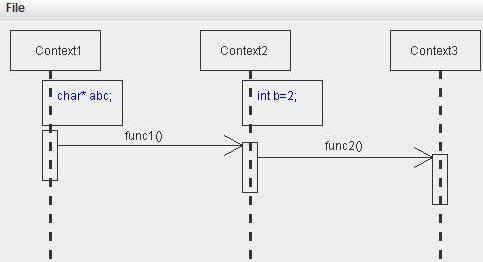
\includegraphics{styles/Error_trace_path.jpg}
	\label{Error_trace_path}
	\caption{Error trace path in UML sequence diagram}
\end{figure}
